\documentclass[submit]{harvardml}



% You don't need to change these.
\course{CS181-S18}
\assignment{Assignment \#2 v1.1}
\duedate{11:59pm Feb 23rd, 2018}

\usepackage[OT1]{fontenc}
\usepackage[colorlinks,citecolor=blue,urlcolor=blue]{hyperref}
\usepackage[pdftex]{graphicx}
\usepackage{subfig}
\usepackage{fullpage}
\usepackage{amsmath}
\usepackage{amssymb}
\usepackage{color}
\usepackage{soul}
\usepackage{todonotes}
\usepackage{listings}
\usepackage{common}
\usepackage{bm}
\usepackage{relsize}
\usepackage{float}

\usepackage[mmddyyyy,hhmmss]{datetime}
    


\definecolor{verbgray}{gray}{0.9}
\definecolor{answergreen}{rgb}{0.09,0.42,0.31}

\lstnewenvironment{csv}{%
  \lstset{backgroundcolor=\color{verbgray},
  frame=single,
  framerule=0pt,
  basicstyle=\ttfamily,
  columns=fullflexible}}{}



\newenvironment{answer}{%
    \color{answergreen}\bf}
  {%
  }

\begin{document}
%\newcommand{\FT}{\mathcal{F}}
\newcommand{\bx}{\mathbf{x}} %%%% WARNING: may cause unexpected behavior
\newcommand{\bX}{\mathbf{X}} %%%% WARNING: may cause unexpected behavior
\newcommand{\by}{\mathbf{y}} %%%% WARNING: may cause unexpected behavior

\newcommand{\bw}{\mathbf{w}} %%%% WARNING: may cause unexpected behavior
\newcommand{\bS}{\mathbf{S}} %%%% WARNING: may cause unexpected behavior

\newcommand{\mBI}{\mathbb{I}_{ik}} %%%% WARNING: may cause unexpected behavior
%\newcommand{\bpi}{\mathbf{\pi}} %%%% Already built into latex 

%\newcommand{\bmu}{\mathbf{\mu}} %%%% Already built into latex 
\newcommand{\bvar}{\mathbf{\sigma}^2} %%%% WARNING: may cause unexpected behavior
\newcommand{\bSig}{\mathbf{\Sigma}} %%%% WARNING: may cause unexpected behavior
\newcommand{\lsum}{\mathlarger{\sum}} %%%% WARNING: may cause unexpected behavior


% \newcommand{\*x}{\mathbf{x}} %%%% apparently not a thing in latex.


%%% Change the assignment details here:
{
  \begin{center}
{\Large Homework 2: Bayesian Methods and Multiclass Classification}\\
\end{center}
}
\subsection*{Introduction}

This homework is about Bayesian methods 
and  multiclass classification. In lecture we have
primarily focused on binary classifiers trained to discriminate
between two classes. In multiclass classification, we discriminate
between three or more classes. We encourage you to first read the
Bishop textbook coverage of these topic, particularly: Section 4.2
(Probabilistic Generative Models), Section 4.3 (Probabilistic
Discriminative Models).
%, and, if MLE is troublesome, review 
%the materal Section 1
%and lecture 3.


As usual, we imagine that we have the input matrix $\boldX \in
\reals^{n \times m}$ (or perhaps they have been mapped to some basis
$\bm{\Phi}$, without loss of generality) but our outputs are now
``one-hot coded''.  What that means is that, if there are~$c$ output
classes, then rather than representing the output label $y$ as an
integer~${1,2,\ldots,c}$, we represent $\boldy$ as a binary vector of
length~$c$. These vectors are zero in each
component except for the one corresponding to the correct label, and
that entry has a one.  So, if there are 7 classes and a particular
datum has label 3, then the target vector would be~${C_3 = [0,0,1,0,0,0,0]}$. 
If there are $c$ classes, the set of possible outputs is $\{C_1 \ldots C_c \} = \{C_k\}_{k=1}^c$.
Throughout the assignment we will assume
that output $\boldy \in \{C_k\}_{k=1}^c$.\\

The problem set has three problems: 
\begin{itemize}
\item In the first problem, you will explore the properties of Bayesian
estimation methods for the Bernoulli model as well as the special
case of Bayesian linear regression with a simple prior.
%
\item  In the second
problem, you will dive into  matrix algebra and the methods behind
generative multiclass classifications. You will extend the discrete classifiers  
that we see in  lecture to a Gaussian model.
%
\item Finally, in the third problem, you will implement 
 logistic regression as well as a generative classifier 
from close to scratch.
%
\end{itemize}

\newpage
\begin{problem}[Bayesian Methods, 10 pts]

  This question helps to build your understanding of the
  maximum-likelihood estimation (MLE) vs. maximum a posterior estimator
  (MAP) and posterior predictive estimator, first in the
  Beta-Bernoulli model and then in the linear regression setting.\\

First consider the Beta-Bernoulli model (and see lecture 5.) 
%
\begin{enumerate}
\item[1.] Write down the expressions for the MLE, MAP and posterior predictive
distributions, and for
a prior $\theta\sim Beta(4,2)$ on the
parameter of the Bernoulli,
and  with data $D= 0, 0, 1, 1, 0, 0, 0, 0, 1, 0, 1, 1,$ 
$1, 0, 1, 0$, plot 
the three different
estimates after each additional
sample.
%
\item[2.] Plot the posterior distribution (prior for 0 examples) on $\theta$ after 0, 4, 8, 12 and 16
examples. (Using whatever tools you like.)
%
\item[3.] Interpret the differences you see between the three different
estimators.
%
%note, initial skew is to large 1, but data has $\theta=0.4$
%
\end{enumerate}

Second, consider the Bayesian Linear Regression model, with
data $D=\{(\boldx_i,y_i)\}_{i=1}^n$, $\boldx_i\in\mathbb{R}^m$,
 $y_i\in\mathbb{R}$, and generative model 
%
$$
y_i\sim\mcN(\boldw^\top\boldx_i,\beta^{-1})
$$
for (known) precision $\beta$ (which is just the reciprocal
of the variance). Given this, the likelihood of the
data is Consider the special case of 
an isotropic (spherical) prior on weights, with
%
$$
p(\boldw)=\mcN(\boldw|\bold0,\alpha^{-1}\boldI)
$$

This prior makes sense when you have little prior information and do not know much about the relationship among features so you can simplify by assuming independence.

\begin{enumerate}

\item[4.] Using the method in lecture of taking logs, expanding and pushing terms
that don't depend on $\boldw$ into a constant, and finally collecting
terms and completing the square, confirm that the posterior on
weights after data $D$ is $\boldw\sim\mcN(\boldw|\boldm_n,\boldS_n)$,
where
%
\begin{align*}
\boldS_n&=(\alpha\boldI+\beta\boldX^\top\boldX)^{-1}\\
\boldm_n&=\beta\boldS_n\boldX^\top\boldy
\end{align*}
\end{enumerate}
\end{problem}



%%%%%%%%%%%%%%%%%%%%%%%%%%%%%%%%%%%%%%%%%%%%%
% Problem 1 - Worked 
%%%%%%%%%%%%%%%%%%%%%%%%%%%%%%%%%%%%%%%%%%%%%
\newpage
\begin{enumerate}
    \item[1a.] Write down the expressions for the MLE, MAP and posterior predictive distributions

    \begin{answer}
        % As pulled from spring 2017 Lecture 7 notes
        Define $num_0$ and $num_1$ as the number of 0s of and 1s, respectively,
        that we have observed so far.

        $$ MLE = \frac{num_0}{num_0 + num_1} $$

        $$ MAP =  \frac{
            \alpha+ num_1-1}{
            \alpha+\beta+num_0+num_1-2} $$

        $$ Postpred = \frac{
            \alpha+num_1}{
            \alpha+\beta+num_1+num_0}$$

    \end{answer}

    \item[1b.] And for a prior $\theta\sim Beta(4,2)$ on the parameter of the Bernoulli, and with data $D= 0, 0, 1, 1, 0, 0, 0, 0, 1, 0, 1, 1, 1, 0, 1, 0$, plot the three different estimates after each additional
sample.
    \begin{answer}

        Plot of estimate for the $\theta_{MLE}$, $\theta_{MAP}$, and posterior predictive, after each of 16 observations.
    \begin{figure}[H] \centering
        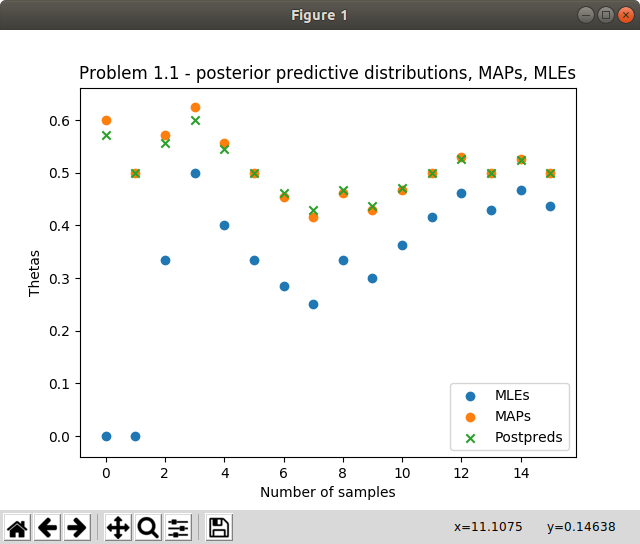
\includegraphics[width=0.5\textwidth]{Problem1-1.png}
        % yea it's a screenshot. 'sbecause I wanted to deal with a reasonable
        % file manager GUI for saving the image
        % Maybe I should have smoothed a line over the points, to make it
        % clearer what's going on
            \caption{}
            \label{Problem 1, part 1.} %fig:posterior_distro}
    \end{figure}


%The posterior predictive gives us a guess for what value we might observe going forward, based on the observations so far (modeled as being a Bernoulli process) and our prior (modeled as a Beta distribution) 
    \end{answer}
%
\item[2.] Plot the posterior distribution (prior for 0 examples) on $\theta$ after 0, 4, 8, 12 and 16
examples. (Using whatever tools you like.)
%
    \begin{answer}

Posterior distribution on theta (with initial zero prior) on $\theta$, after obtaining 0,4,8,12, and 16 samples

    \begin{figure}[H] \centering
        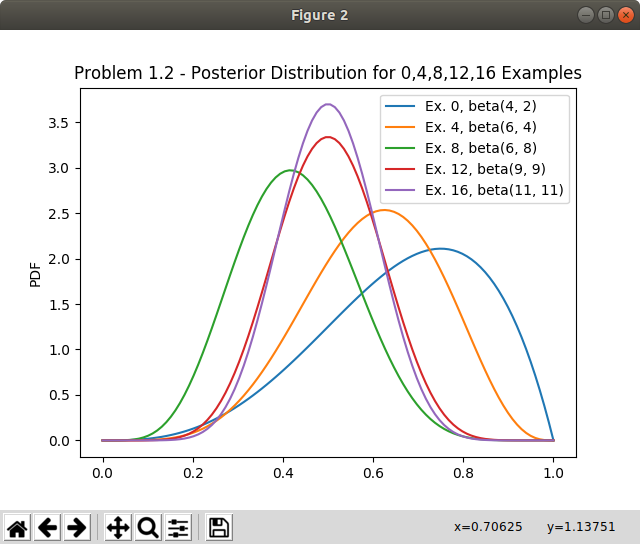
\includegraphics[width=0.5\textwidth]{Problem1-2.png}
        % yea it's a screenshot. 'sbecause I wanted to deal with a reasonable
        % file manager GUI for saving the image
        % Maybe I should have smoothed a line over the points, to make it
        % clearer what's going on
            \caption{Problem 1, part 2.}
        \label{fig:theta_obs} %fig:posterior_distro}
    \end{figure}
    \end{answer}


\item[3.] Interpret the differences you see between the three different estimators.

\begin{answer} 
    % Bishop chapter 1.2.5 MAP (pg 30)
    % Bishop chapter 2.1 Beta distribution
    % Spring 2017 Lecture 5
    We have defined the posterior distribution as equal to $Bernoulli(\theta)
    \cdot Beta(\alpha, \beta)$.  The Bernoulli distribution is the generative
    model, or \textit{likelihood} of our data occurring (given this distribution) and the
    Beta distribution is our \textit{prior}, where we weigh the new observations 
    against our prior belief about the system.

    We started with an initial prior (in blue on Figure \ref{fig:theta_obs},
    which lends us to believe that the Bernoulli process we're observing is
    skewed toward producing ones, that is the $\theta$ parameter characterizing
    the distribution is fairly large.

    Note: In a Bernoulli distribution $\theta$ is the likelihood of seeing a one
    and $1-\theta$ is the likelihood of seeing a zero.

    Our maximum likelihood estimates do not incorporate a prior belief. Thus
    $\theta_MLE$ exactly matches the initial two data points, zero. In contrast,
    our maximum posteriors (MAPs), incorporate prior belief. Thus, although we
    see two zeros, our MAP remains high. The posterior prediction incorporates
    our uncertainty about w into our prediction. It tends to estimate a value
    between the MAP and MLE, converging to the MAP prediction as the prior on
    the MAP updates. Over time, the MLE also converges to the MAP since the
    counts on average will equal the mean of the generative distribution.

    We can actually see this on the Figure \ref{fig:theta_obs}. Initially our
    mean on the prior is skewed to the right, but as we get more samples, we
    update the prior so that it shifts to average around 0.5. Additionally, as
    we get observation data, we become more confident about the shape of our
    generative distribution, and thus the variance on the beta distribution goes down. 
    % FIN.

    % ?? Why is there a postpred estimate *above* the MAP?

    % Full bayes vs MAP: posterior predictive considers uncertainty on w when
    % making a prediction

    % MAP = most probable of $w$ given the data, aka maximizing the posterior
    % distribution
    % todo: go over section 3 notes about difference between posterior
    % predictive and posterior, both are distributions... What would concrete
    % example be in this case -- one is distribution over theta of
    % Bernoulli, one is distribution over expected values given our uncertainty
    % in our prior

\end{answer}


% do: work this out without reference section 3 notes at all
\item[4.]
Given likelihood
$$p(\boldy|\boldX,\boldw) = \mcN(\boldy|\boldX\boldw,\beta^{-1}\mathbf{I})$$
and prior     
$$ p(\boldw)=\mcN(\boldw|\bold0,\alpha^{-1}\boldI) $$
    
Confirm that the posterior on weights after data $D$ is 
$$\boldw\sim\mcN(\boldw|\boldm_n,\boldS_n)$$
where $\boldS_n =(\alpha\boldI+\beta\boldX^\top\boldX)^{-1}i$ and 
$\boldm_n=\beta\boldS_n\boldX^\top\boldy$.

Do so by [1] taking logs 
[2] expanding and pushing terms that don't depend on $\boldw$ into a constant
[3] finally collecting terms and completing the square

% xianzai

\begin{answer}
   % As per [1] Taking logs: 
    At a high level, the posterior equals the likelihood times
    the prior. 
    
    After taking the natural log of the posterior, 
    we get $$ \ln p(\bw|D) \propto \ln p(\by|\bX,\bw) + \ln p(\bw) $$

    %As per [2] 
    We expand using the definition of the normal distribution, as applied to
    the likelihood and prior. 

    ~~ Note that
    \begin{equation}
     \mathcal{N}(\boldsymbol x \mid \boldsymbol\mu, \Sigma)
             = \frac{1}{\sqrt{(2\pi)^D|\boldsymbol\Sigma|}}  \exp\left(-\frac 1 2 ({\mathbf x}-{\boldsymbol\mu})^\mathrm{T}{\boldsymbol\Sigma}^{-1}({\mathbf x}-{\boldsymbol\mu})\right)
    \end{equation}

    And that the natural log is equal to 
    \begin{equation}
     - \frac{1}{2} \left( D \ln2\pi + \ln|\bSigma| + (\bx - \bmu)^T
        \bSigma^{-1} (\bx-\bmu) \right) \label{lnNormal}
    \end{equation}
   ~~ 
    
    % per [3] 
    % VIM: no % in visual substitution
    Plugging in and pushing terms that don't depend on $\bw$ into a constant, we get 
    \begin{align*}
        \ln p(\bw|D) &\propto  \\
        &=-\frac{1}{2} (\by-\bX\bw)^T \beta(\by-\bX\bw) - \frac{1}{2}
        (\bw-0)^T(\alpha^{-1}I)^{-1}(\bw-0) \\
        &=- \frac{\beta}{2}(\by-\bX\bw)^T(\by-\bX\bw) - \frac{\alpha}{2}\bw^T\bw
   \end{align*}

       FOILing, and dropping the first term which doesn't  depend on $\bw$ ;
       and on the second line noting that $\by^T\bX\bw = \bw^T\bX^T\by$ as well
       as carrying out the transpose, we get
   \begin{align}
           &= - \frac{\beta}{2}     \left( - \by^T \bX\bw - (\bX\bw)^T \by + (\bX\bw)^T
           \bX\bw \right) 
           - \frac{\alpha}{2} \bw^T\bw \\
           % uh... there's someting fishy here about X^T * w vs X^T * w
           % latex makes it really annoying to keep moving between per datapoint
           % and per vector of data....  this is a little fishy but don't have
           % time to fix
        &=- \frac{1}{2}\left(- 2 \beta(\bw^T \bX^T\by) + \beta(\bw^T\bX^T\bX\bw) - \alpha
        \bw^T\bw \right) \\
        &= - \frac{1}{2} \left( -2\bw^T(\beta \bX^T\by)- \bw^T(\beta \bX^T\bX -
        \alpha)\bw
        \right) \label{target1}
        % create aligned, numbered equation, while bumping up internal eqn
        % counter in latex
    \end{align}

    Now working backwards, we note that we would like to show that
    $\boldw\sim\mcN(\boldw|\boldm_n,\boldS_n)$. Doing as before (taking the log
    and expanding), we get that our target equation is... (on third line,
    dropping term without w, and combining two middle terms) 
    \begin{align}
        &= - \frac{1}{2} \left( (\bw-\mathbf{m}_n)^T \bS_n^{-1} (\bw-\mathbf{m}_n) \right) \\
        &= - \frac{1}{2} ( \bw^T\bS_n^{-1}\bw - \mathbf{m}_n^T\bS_n^{-1}\bw -
        \bw^T\bS_n^{-1}\mathbf{m}_n 
        + \mathbf{m}_n^T\bS_n^{-1}\mathbf{m}_n ) \\
        &= -\frac{1}{2} (\bw^T\bS_n^{-1}\bw - 2\bw^T\bS_n^{-1}\mathbf{m}_n)  \\ % todo: work out why the middle two terms are equivalent
        \label{target2} 
    \end{align}

    Looking above at Equation \ref{target1} we see that it is of similar form
    to Equation \eqref{target2} above, if we define 
    $$ \bS_n = (\alpha\mathbf{I} + \beta \bX^T \bX)^{-1} $$ 
    $$ \bS_n^{-1}\mathbf{m}_n = \beta \bX^T \by$$

    For the last equation, Shifting $S_n$ to the other side we get
    $$ \mathbf{m}_n = \beta \bS_n \bX^T \by $$
    as we were asked to prove.

    % FIN.





\end{answer}
\end{enumerate}


%\subsection*{2. Mooooar matrix calculus [10 pts]}
%%%%%%%%%%%%%%%%%%%%%%%%%%%%%%%%%%%%%%%%%%%%%
% Problem 2
%%%%%%%%%%%%%%%%%%%%%%%%%%%%%%%%%%%%%%%%%%%%%
\begin{problem}[Return of matrix calculus, 10pts]

  Consider now a generative $c$-class model.  We adopt class prior
  $p(\boldy = C_k; \bpi) = \pi_k$ for all $k \in \{1, \ldots, c\}$
(where $\pi_k$ is a parameter of the prior).
%
%that define the prior. 

%5% xianzai
Let  $p(\boldx|\boldy=C_k)$ denote
the class-conditional density of features $\boldx$ (in this
case for class $C_k$). Consider the data set $D = \{(\boldx_i,
\boldy_i)\}_{i=1}^n$ where as above $\boldy_i \in \{C_k\}_{k=1}^c$ is
encoded as a one-hot target vector. 
%
\begin{enumerate}
  \item Write out the negated log-likelihood of the data set,
    $-\ln p(D ; \bpi)$.
%
  \item Since the prior forms a distribution, it has the constraint that
    $\sum_k\pi_k - 1 = 0$.  Using the hint on
Lagrange multipliers below, give the
    expression for the maximum-likelihood estimator for the prior
    class-membership probabilities, i.e.
    $\hat \pi_k.$
    Make sure to write out the intermediary equation you need
    to solve to obtain this estimator. Double-check your answer: the final
    result should be very intuitive!
\end{enumerate}

    For the remaining questions, let the 
    class-conditional probabilities be Gaussian distributions with 
the same covariance matrix
    $$p(\boldx | \boldy = C_k) = \mathcal{N}(\boldx |  \bmu_k, \bSigma), \text{\ for\ }k \in \{1,\ldots, c\}$$
%
and different means $\bmu_k$ for each class.
%
    \begin{enumerate}
  \item[3.] Derive the gradient of the negative log-likelihood with respect to vector $\bmu_k$.
    Write the expression in matrix form as a function of the variables defined
    throughout this exercise. Simplify as much as possible for full credit.
  \item[4.] Derive the maximum-likelihood estimator for vector $\bmu_k$. Once
    again, your final answer should seem intuitive.
  \item[5.] Derive the gradient for the negative log-likelihood with respect to the
    covariance matrix $\bSigma$ (i.e., looking
to find an MLE for the covariance). 
Since you are differentiating with respect to a
    \emph{matrix}, the resulting expression should be a matrix!
%
  \item[6.] Derive the maximum likelihood estimator of the covariance matrix.
\end{enumerate}

\paragraph{Hint: Lagrange Multipliers.} Lagrange Multipliers are a method for
optimizing a function $f$ with respect to an
equality constraint, i.e. 
\[\min_{\boldx} f(\boldx)\ \text{s.t.}\ g(\boldx) = 0.\]

This can be turned into an unconstrained problem by introducing a
Lagrange multiplier $\lambda$ and constructing the Lagrangian function,
\[L(\boldx, \lambda) =  f(\boldx) + \lambda g(\boldx).\]

It can be shown that it is a necessary condition that the optimum 
is a critical point of this new function. We can find this point by solving two equations:

\[\frac{\partial L(\boldx, \lambda)}{\partial  \boldx} = 0  \ \ \text{and}\  \  \frac{\partial L(\boldx, \lambda)}{\partial \lambda} = 0 \]


\paragraph{Cookbook formulas.} Here are some formulas you might want to consider
using to compute difficult gradients. You can use them  in the homework
without proof. If you are looking to hone your matrix calculus skills, try to
find different ways to prove these formulas yourself (will not be part of the
evaluation of this homework). In general, you can use any formula from the matrix cookbook,
as long as you cite it. We opt for the following common notation:
$\boldX^{-\top} := (\boldX^{\top})^{-1}$
\begin{align*}
  & \frac{\partial \bolda^\top \boldX^{-1} \boldb}{\partial \boldX} = - \boldX^{-\top} \bolda \boldb^\top \boldX^{-\top} \\
  & \frac{\partial \ln | \det (\boldX) |}{\partial \boldX} = \boldX^{-\top}
 \end{align*}
 \end{problem}



\newpage


%%%%%%%%%%%%%%%%%%%%%%%%%%%%%%%%%%%%%%%%%%%%%
% Problem 2 - Worked 
%%%%%%%%%%%%%%%%%%%%%%%%%%%%%%%%%%%%%%%%%%%%%
\begin{enumerate}
    \item[1.] Write out the negated log-likelihood of the data set

    \begin{answer}

        The likelihood of the dataset occuring is the product of the
        probabilities of each datapoint occuring.
        $$P(D;\bpi_k) = \prod_{i=1}^n P(x_i, y_i)$$

        By definition, the joint probability
        $$P(\bx,\by) = p(\by) p(\bx|\by)$$

        %In english, our dataset likelihood equals
        %our class probability (aka our class prior) times our class conditional.  
        %class prior = our belief about the shape of the distributions for each class 
        %class conditional = our belief about how likely any datapoint is in any
        %class
        % e.g. how many cat datapoints are in our dataset 

        We are given that:  \\
        the class prior $p(\by=C_k; \bpi) = \pi_k$  \\
        the class conditional $p(\bx|\by = C_k)$ 

        Furthermore, we know that there are $c$ classes.  Thus we can write the likelihood 
        %We need the likelihood of any particlar datapoint belonging to any particular dataset. 
        $$p(D; \bpi) = \prod_{i=1}^n \prod_{k=1}^c \pi_k p(x_i | C_k)$$
       
        To find the negative log likelihood (lnll), we take (as stated) the
        log of both sides

        (Note that we use a mathematical notation trick to ensure that we can
        cleanly write the negative lnll. We use $\mathbb{I}\{y_i = k\}$ to indicate that
       for the likelihood, we only want to evaluate the probability $p( \bx, y)$
        for $\bx$'s true class, rather than all classes. To clean things up even
        further, we'll shorten it to $\mBI$ which evaluates to 1 for the $ith$ datapoint's true class k, and zero
        otherwise.)
        \begin{align}
            - \ln p(D; \bpi) &=  \sum_{i=1}^n \sum_{k=1}^c \mBI 
                 [\ln(\pi_k) - \ln p(x_i|C_k) ]\\
                &= - \sum_{i=1}^n \sum_{k=1}^c \mBI [
                    \ln(\pi_k) - \ln p(x_i| y_i = C_k) ]  \label{lnLL}
        \end{align}
    % FIN.
    \end{answer}

    \item[2.1]  Using the hint on Lagrange multipliers below, give the
    expression for the maximum-likelihood estimator for the prior
    class-membership probabilities, i.e.  $\hat \pi_k.$

    \begin{answer}

        To find the MLE for $\hat \pi_k$, we take the derivative of the
        likelihood function with respect to $\pi_k$. 
        
        \begin{align}
            %%
            \arg\max_{\bpi_k} 
            -\ln L(D) 
            &= \arg\max_{\bpi_k} 
                 - \sum_{i=1}^n \sum_{k=1}^c \mBI [
                    \ln(\pi_k) - \ln p(x_i| y_i = C_k) ]\\
            &= \arg\max_{\bpi_k} 
                 - \sum_{i=1}^n \sum_{k=1}^c \mBI 
                    \ln(\pi_k) \label{lnll}
        \end{align}
        (Note that the class conditional $p(x_i | C_k)$ does \textit{not} depend on
        $\pi_k$, which is a parameter of a completely separate distribution (the
        class prior), and so we have dropped the class conditional term.)

        To find the MLE for $\hat \pi_k$, aka the $\arg\max{\bpi_k}$ of the
        likelihood function, we normally set the derivative (with respect to
        $\bpi_k$) equal to zero and solve for $\bpi_k$. However, note
        that as we have multiple $\bpi$ parameters (one for each class), we must
        include the constraint that $\sum_{k=1}^c \pi_k-1=0$.

        We will use the method of Lagrange multipliers to handle this extra
        constraint when solving for $\hat \pi_k$.
            
        Substituting equation \eqref{lnll}, and our constraint, into the
        following equation (where $g(\bx)$ is the constraint function)
        $$
        Lag(\bx,\lambda) = f(\bx)+\lambda g(\bx) \\
        $$
        we get
        $$
        Lag(\bpi,\lambda) 
            = - \lsum_{i=1}^n \lsum_{k=1}^c \mBI \ln(\pi_k) + \lambda( \sum_{k=1}^c\pi_k-1)
        $$
        $$
        Lag(\pi_k,\lambda) 
            = - \lsum_{i=1}^n \mBI \ln(\pi_k) + \lambda( \sum_{k=1}^c\pi_k-1)
            $$

        To find the optimum, we then solve the system of two equations  

        \begin{equation*}
            \frac{\partial}{\partial \bpi} Lag(\bpi_k,\lambda)=0 \text{ and }
        \frac{\partial}{\partial\lambda} Lag(\bpi_k, \lambda)= 0.
        \end{equation*}
        
        %%% SEE: kroenicker delta
        Note that we can "remove" the summation over k because we are taking the
        derivative with respect to all individual $pi_k$'s, as a vector, and the
        indicator allows us to only care about the $k$th class.
        % uh, is this really true? it seems reasonable

        $$
        \frac{\partial}{
            \partial \pi_k} Lag(\bpi,\lambda) = -\sum_{i=1}^n \frac{1}{\pi_k} - \lambda = 0
        $$

        The indicator $\mBI$ says that we only care about the points in the $k$
        class, which we will denote as $N_k$. We may thus pull the $\pi_k$ out
        of the summation, and get $N_k \pi_k$. Thus we solve and get

        $$ \pi_k = - \frac{\lambda}{N_k} \\ $$

        From the second derivative, we get

        $$
        \frac{\partial}{
            \partial \lambda} Lag(\bpi,\lambda) =  \sum_{k=1}^c\pi_k-1 = 0
        $$

       Combining the two equations, we may write that 

        $$
        \sum_{k=1}^c - \frac{\lambda}{N_k}= 1
        $$
        Note that $\lambda$ is a constant, while the sum across all classes of the
        number of points in each class is $n$. Simplifying we get that 
        \begin{align*}
            -\lambda \sum_{k=1}^c \frac{1}{N_k} &= 1\\
            -\lambda \frac{1}{n} &= 1 \\
            \lambda &=  -n
        \end{align*}

        Thus we get that for each class, the prior on $y_k$, or our belief about
        the distribution of $y_k$, is simply the percent of datapoints in that
        $k$ class over the total number of datapoints $n$.

        $$ \pi_k = \frac{n}{N_k}
        $$

        % FIN.
    \end{answer}
        

    Make sure to write out the intermediary equation you need to solve to obtain this estimator. 

    Double-check your answer: the final result should be very intuitive!

    %\xianzai
  \item[3.] Derive the gradient of the negative log-likelihood with respect to vector $\bmu_k$.
    Write the expression in matrix form as a function of the variables defined
    throughout this exercise. Simplify as much as possible for full credit.
    
    \begin{answer}
        We will use the expression for negative log-likelihood (lnLL) in
        \eqref{lnLL}. We plug in the class-conditional distribution we were
        given 
    $$p(\boldx | \boldy = C_k) = \mathcal{N}(\boldx |  \bmu_k, \bSigma)$$
        into the equation for the natural log of the normal distribution \eqref{lnNormal}
        to get our $L_g$ equation
        \begin{equation}
            \sum_{i=1}^n \sum_{k=1}^c \mBI \left[ 
            -\frac{1}{2} (
                \ln|\bSigma|+(\bx_i-\bmu_k)^T\Sigma^{-1} (\bx_i-\bmu_k) )
                + \ln\pi_k \right] \label{lnGaussLL}
        \end{equation}
        Dropping terms without $\mu_k$ we get 
        \begin{equation}
            \sum_{i=1}^n \sum_{k=1}^c \mBI 
            \left[ -\frac{1}{2} (\bx_i-\bmu_k)^T \Sigma^{-1} (\bx_i-\bmu_k) 
            \right] + const
        \end{equation}
        Using the chain rule, we can say that 
        $$
        \frac{\partial L_g}{\partial \bmu_k} = 
        \frac{\partial L_g}{\partial( \bx_n - \bmu_k)} 
        \frac{\partial(\bx_n - \bmu_k)}{\partial \bmu_k} 
        = - \frac{\partial L_g}{\partial( \bx_n - \bmu_k)} 
        $$
        Using the formula
        %$$  \frac{\partial \mathbf{a}^T \bX^{-1} \mathbf{b}}{\partial \bX}  
        %= - \bX^{-T} \mathbf{a} \mathbf{b}^T \bX^{-T}
        %$$
        $$  \frac{\partial \mathbf{a}^T \bX \mathbf{a}}{\partial \bX}  
             = \frac{\partial \mathbf{a}^T \bX^T \mathbf{a}}{\partial \bX}  
            = \mathbf{a}^T\mathbf{a}
        $$
        %% is this really true? why is a^T X A == a^T X^T a ?
        we get 
        $$
        \frac{\partial L_g}{\partial \bmu_k} = \frac{1}{2} 
             \sum_{i=1}^n \sum_{k=1}^c \mBI  \left[ 
             (\bSigma^{-1} + \bSigma^{-T})
             (\bx_n - \bmu_k) \right]
        $$
        For cleanliness the covariances can be pulled out of the summations so that we get 
        \begin{equation}
        \frac{\partial L_g}{\partial \bmu_k} = \frac{1}{2} 
             (\bSigma^{-1} + \bSigma^{-T})
             \sum_{i=1}^n \sum_{k=1}^c \mBI 
             (\bx_n - \bmu_k)  \label{MLEmu}
        \end{equation}

    \end{answer}

  \item[4.] Derive the maximum-likelihood estimator for vector $\bmu_k$. Once
    again, your final answer should seem intuitive.

    \begin{answer}
        To get the MLE for $\bmu_k$ We set the gradient in \eqref{MLEmu} equal to zero and
        solve for $\bmu_k$.
        $$
         0 = \frac{1}{2} 
             (\bSigma^{-1} + \bSigma^{-T})
             \sum_{i=1}^n \sum_{k=1}^c \mBI 
             (\bx_i - \bmu_k) 
             $$
             $$
         0 = \sum_{i=1}^n \sum_{k=1}^c \mBI 
             (\bx_i - \bmu_k) 
        $$

        Thinking carefully, we see that the sum of $\mu_k$ across all the
        points in that class, is equal to $N_k \mu_k$. Thus we can pull the
        $\mu_k$ out of the indicator and summation to get $N_k \cdot \mu_k$.
        Furthermore we see that since we are solving with respect to the $k$th
        class, we can indicate with a $k$ subscript that that is the x we care
        about and remove the indicator for clarity.

        Thus we get that 
        $$ 
        0 = N_k \mu_k - \lsum_{i=1}^n \bx_n
        $$
        And therefore we end up with
        \begin{equation}
            \bmu_k = \frac{1}{N_k} \lsum_{i=1}^n \bx_n
        \end{equation}

        In other words, that the mean of the distribution is the sum of the
        value of all the datapoints in the class, divided by the number of datapoints in the
        class.
        % FIN.
    \end{answer}

  \item[5.] Derive the gradient for the negative log-likelihood with respect to the
    covariance matrix $\bSigma$ (i.e., looking to find an MLE for the covariance). 
    Since you are differentiating with respect to a \emph{matrix}, the resulting expression should be a matrix!

 \begin{answer} 
     As before we start with our $L_g$ as derived in \eqref{lnGaussLL}.
        \begin{equation}
            \sum_{i=1}^n \sum_{k=1}^c \mBI \left[ 
            -\frac{1}{2} (
                \ln|\bSigma|+(\bx_i-\bmu_k)^T\Sigma^{-1} (\bx_i-\bmu_k) )
                + \ln\pi_k \right] 
        \end{equation}
        Dropping terms without $\bSigma$ we get
        \begin{equation}
            \sum_{i=1}^n \sum_{k=1}^c \mBI \left[ 
            -\frac{1}{2} (
                \ln|\bSigma|+(\bx_i-\bmu_k)^T\Sigma^{-1} (\bx_i-\bmu_k) )
                \right] 
        \end{equation}


        Taking the partial derivative, we get 
        \begin{equation}
        \frac{\partial L_g}{\partial \bSigma} = 
            \sum_{i=1}^n \sum_{k=1}^c \mBI \left[ 
            -\frac{1}{2} (
                \ln|\bSigma|+(\bx_i-\bmu_k)^T\Sigma^{-1} (\bx_i-\bmu_k) )
                \right] 
        \end{equation}

        Using the equations as given to us
    \begin{align*}
      & \frac{\partial \bolda^\top \boldX^{-1} \boldb}{\partial \boldX} = - \boldX^{-\top} \bolda \boldb^\top \boldX^{-\top} \\
      & \frac{\partial \ln | \det (\boldX) |}{\partial \boldX} = \boldX^{-\top}
     \end{align*}

     We get 
        \begin{equation}
        \frac{\partial L_g}{\partial \bSigma} = 
            \sum_{i=1}^n \sum_{k=1}^c \mBI \left[ 
            -\frac{1}{2} (
            \bSigma^{-T} + \bSigma^{-T} (\bx_i - \bmu_k)^T (\bx_i - \bmu_k)
            \bSigma^{-T} )
                \right]  \label{gradsig}
        \end{equation}


        % FIN.
 \end{answer}
  \item[6.] Derive the maximum likelihood estimator of the covariance matrix.

      \begin{answer}
      Setting  \eqref{gradsig} equal to 0 and solving we get 

        \begin{equation}
            \sum_{i=1}^n \sum_{k=1}^c \mBI \bSigma^{-T} =
            \sum_{i=1}^n \sum_{k=1}^c \mBI \bSigma^{-T} (\bx_i - \bmu_k)^T (\bx_i - \bmu_k)
            \bSigma^{-T} 
        \end{equation}


        Left and right multiplying (on both sides of the equation) by
        $\Sigma^{T}$ we get 

        $$
          N \Sigma ^T =  
            \sum_{i=1}^n \sum_{k=1}^c \mBI (\bx_i - \bmu_k)^T (\bx_i - \bmu_k)
            $$

            Taking the transpose of both sides, finally we get that 
        $$
          \Sigma  =   \frac{1}{N}
            \sum_{i=1}^n \sum_{k=1}^c \mBI (\bx_i - \bmu_k)^T (\bx_i - \bmu_k)
            $$
      \end{answer}


\end{enumerate}




%%%%%%%%%%%%%%%%%%%%%%%%%%%%%%%%%%%%%%%%%%%%%
% Problem 3 - 
%%%%%%%%%%%%%%%%%%%%%%%%%%%%%%%%%%%%%%%%%%%%%


\subsection*{3. Classifying Fruit [15pts]}
You're tasked with  classifying three different kinds of fruit, based on their
heights and widths.  Figure~\ref{fig:fruit} is a plot of the data.  Iain Murray
collected these data and you can read more about this on his website at
\url{http://homepages.inf.ed.ac.uk/imurray2/teaching/oranges_and_lemons/}.  We
have made a slightly simplified (collapsing the subcategories together) version
of this available as \verb|fruit.csv|, which you will find in the Github repository.
The file has three columns: type (1=apple, 2=orange, 3=lemon), width,
and height.  The first few lines look like this:
\begin{csv}
fruit,width,height
1,8.4,7.3
1,8,6.8
1,7.4,7.2
1,7.1,7.8
...
\end{csv}
\begin{figure}[h]
\centering
\includegraphics[width=0.5\textwidth]{fruit}
\caption{Heights and widths of apples, oranges, and lemons.  These fruit were
purchased and measured by Iain Murray:
\url{http://homepages.inf.ed.ac.uk/imurray2/teaching/oranges_and_lemons/}.}
\label{fig:fruit}
\end{figure}
\begin{problem}[Classifying Fruit, 15pts]
  You should implement the following:
\begin{itemize}
\item The three-class generalization of logistic regression, also
  known as softmax regression, for these data. You will do this by implementing
  gradient descent on the negative log likelihood. You will need to find good values for the learning rate $\eta$ and regularization strength $\lambda$. See the third practice problem in the section 3 notes for information about multi-class logistic regression, softmax, and negative log likelihood.
%
\item A generative classifier with Gaussian
  class-conditional densities, as in Problem~3. In particular, make
  two implementations of this, one with a shared covariance matrix
  across all of the classes, and one with a separate covariance being
  learned for each class.  Note that the staff implementation can
  switch between these two by the addition of just a few lines of
  code. In the separate covariance matrix case, the MLE for the
  covariance matrix of each class is simply the covariance of the data
  points assigned to that class, without combining them as in the
  shared case.
\end{itemize}
You may use anything in  \texttt{numpy} or \texttt{scipy}, except for \texttt{scipy.optimize}. That being said, if you happen to find a function in \texttt{numpy} or \texttt{scipy} that seems like it is doing too much for you, run it by a staff member on Piazza. In general, linear algebra and random variable functions are fine. The controller file is \texttt{problem3.py}, in which you will specify hyperparameters. The actual implementations you will write will be in \texttt{LogisticRegression.py} and \texttt{GaussianGenerativeModel.py}.


You will be given class interfaces for \texttt{GaussianGenerativeModel} and \texttt{LogisticRegression} in the distribution code, 
and the code will indicate certain lines that you should not change in your final submission. Naturally, don't change these.
These classes will allow the final submissions to have consistency. There will also be a few hyperparameters that are set to
irrelevant values at the moment. You may need to modify these to get your methods to work.
The classes you implement follow the same pattern as scikit-learn, so they should be familiar to you. The distribution code currently outputs nonsense predictions just to show what the high-level interface should be, so you should completely remove the given \texttt{predict()} implementations and replace them with your implementations.

\begin{itemize}
\item The \texttt{visualize()} method for each classifier will save a plot that will show the decision boundaries. You should include these in this assignment.
\item Which classifiers model the distributions well?
\item What explains the differences?

\end{itemize}

In addition to comparing the decision boundaries of the three models visually:
\begin{itemize}

\item For logistic regression, plot negative log-likelihood loss with iterations on the x-axis and loss on the y-axis for several configurations of hyperparameters. Note which configuration yields the best final loss. Why are your final choices of learning rate ($\eta$) and regularization strength ($\lambda$) reasonable? How does altering these hyperparameters affect convergence? Focus both on the ability to converge and the rate at which it converges (a qualitative description is sufficient).

\item For both Gaussian generative models, report negative log likelihood. In the separate covariance matrix case, be sure to use the covariance matrix that matches the true class of each data point.

\end{itemize}

Finally, consider a fruit with width 4cm and height 11cm.  To what
class do each of the classifiers assign this fruit? What do these results tell you about the classifiers' ability to generalize to new data?  Repeat
for a fruit of width 8.5cm and height 7cm.

\end{problem}

\newpage
\subsection*{Calibration [1pt]}
Approximately how long did this homework take you to complete?

Between 60 to 80 hours, depending on if you count pre-readings

\subsection*{Name, Email, and Collaborators}

Name: Nao Ouyang

Email: nouyang@g.harvard.edu    

Collaborators:
Eric
Wilson
Sharon

They are great

\end{document}
